\documentclass{standalone}
\usepackage{tikz}
\usetikzlibrary{arrows.meta, positioning, calc}

\begin{document}

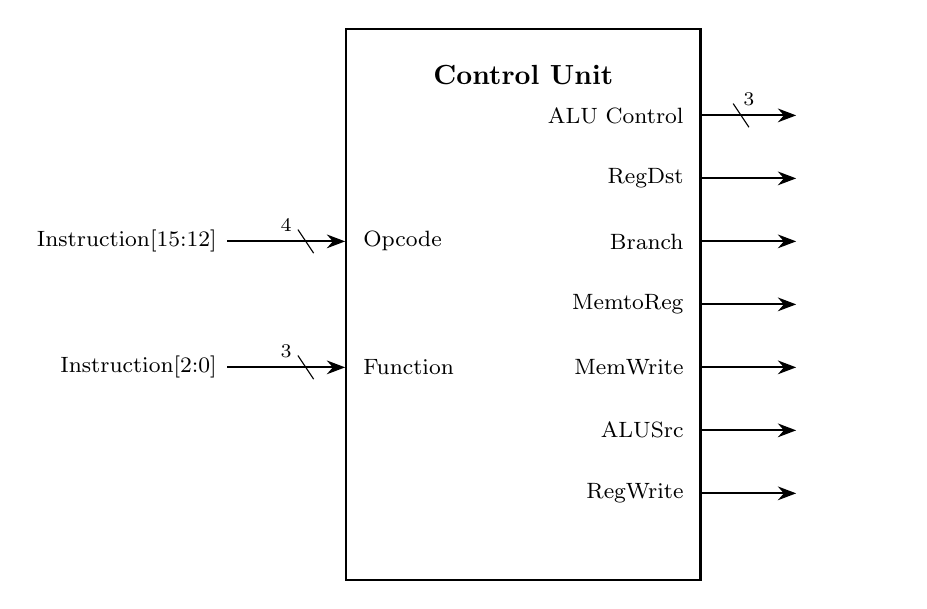
\begin{tikzpicture}[
    box/.style={rectangle, draw, minimum width=4.5cm, minimum height=7.0cm, thick, fill=white},
    port/.style={font=\footnotesize},
    label/.style={font=\scriptsize},
    arrow/.style={->, >=Stealth, thick}
]

    % Main Box (Centered at 0,0)
    \node[box] (ctrl) at (0,0) {};
    
    % Header Title
    \node[font=\bfseries, yshift=-0.6cm] (title) at (ctrl.north) {Control Unit};

    % --- Left Side Inputs ---
    \draw [arrow] ($(ctrl.west)+(-1.5, 0.8)$) -- ($(ctrl.west)+(0, 0.8)$)
        node[pos=0, left, port] {Instruction[15:12]}
        node[midway, above, label] {4}
        node[pos=1, anchor=west, port, xshift=0.1cm] {Opcode};
    \draw ($(ctrl.west)+(-0.6, 0.95)$) -- ($(ctrl.west)+(-0.4, 0.65)$); 

    \draw [arrow] ($(ctrl.west)+(-1.5, -0.8)$) -- ($(ctrl.west)+(0, -0.8)$)
        node[pos=0, left, port] {Instruction[2:0]}
        node[midway, above, label] {3}
        node[pos=1, anchor=west, port, xshift=0.1cm] {Function};
    \draw ($(ctrl.west)+(-0.6, -0.65)$) -- ($(ctrl.west)+(-0.4, -0.95)$);

    % --- Right Side Outputs ---
    \draw [arrow] ($(ctrl.east)+(0, 2.4)$) -- ($(ctrl.east)+(1.2, 2.4)$)
        node[midway, above, label] {3}
        node[pos=0, anchor=east, port, xshift=-0.1cm] {ALU Control};
    \draw ($(ctrl.east)+(0.4, 2.55)$) -- ($(ctrl.east)+(0.6, 2.25)$);

    \foreach \y/\name in {1.6/RegDst, 0.8/Branch, 0/MemtoReg, -0.8/MemWrite, -1.6/ALUSrc, -2.4/RegWrite} {
        \draw [arrow] ($(ctrl.east)+(0, \y)$) -- ($(ctrl.east)+(1.2, \y)$)
            node[pos=0, anchor=east, port, xshift=-0.1cm] {\name};
    }

    % GHOST PATH: Mirrors the left-side labels to force centering on the box
    % Adjust the 2.5cm if your left labels are even longer
    \path ($(ctrl.east)+(2.5, 0)$); 

\end{tikzpicture}

\end{document}